%% This is an example first chapter.  You should put chapter/appendix that you
%% write into a separate file, and add a line \include{yourfilename} to
%% main.tex, where `yourfilename.tex' is the name of the chapter/appendix file.
%% You can process specific files by typing their names in at the 
%% \files=
%% prompt when you run the file main.tex through LaTeX.
\chapter{Pendahuluan}

%\textbf{Catatan}: Manual ini mengacu pada Ijah Webserver versi 201602231639

\section{Use Case Ijah}
Dalam penggunaan Ijah Webserver, ada tiga skenario contoh kasus \emph{(use case)} penggunaan, yaitu
\begin{itemize}
\item End-to-end (both drug-side dan target-side) input
\item Drug-side only input
\item Target-side only input.
\end{itemize}
Ketiga \emph{use case} ini akan dibahas lebih lanjut pada bab selanjutnya, \nameref{Use Case}.

\section{Masuk ke Ijah Webserver}
Untuk mengakses Ijah Webserver, ketikkan URL ijah.apps.cs.ipb.ac.id pada \emph{address bar} browser dan tekan \textbf{Enter}

Tampilan halaman utama Ijah Webserver adalah sebagai berikut:

\begin{figure}[!h]
	\centering
	% 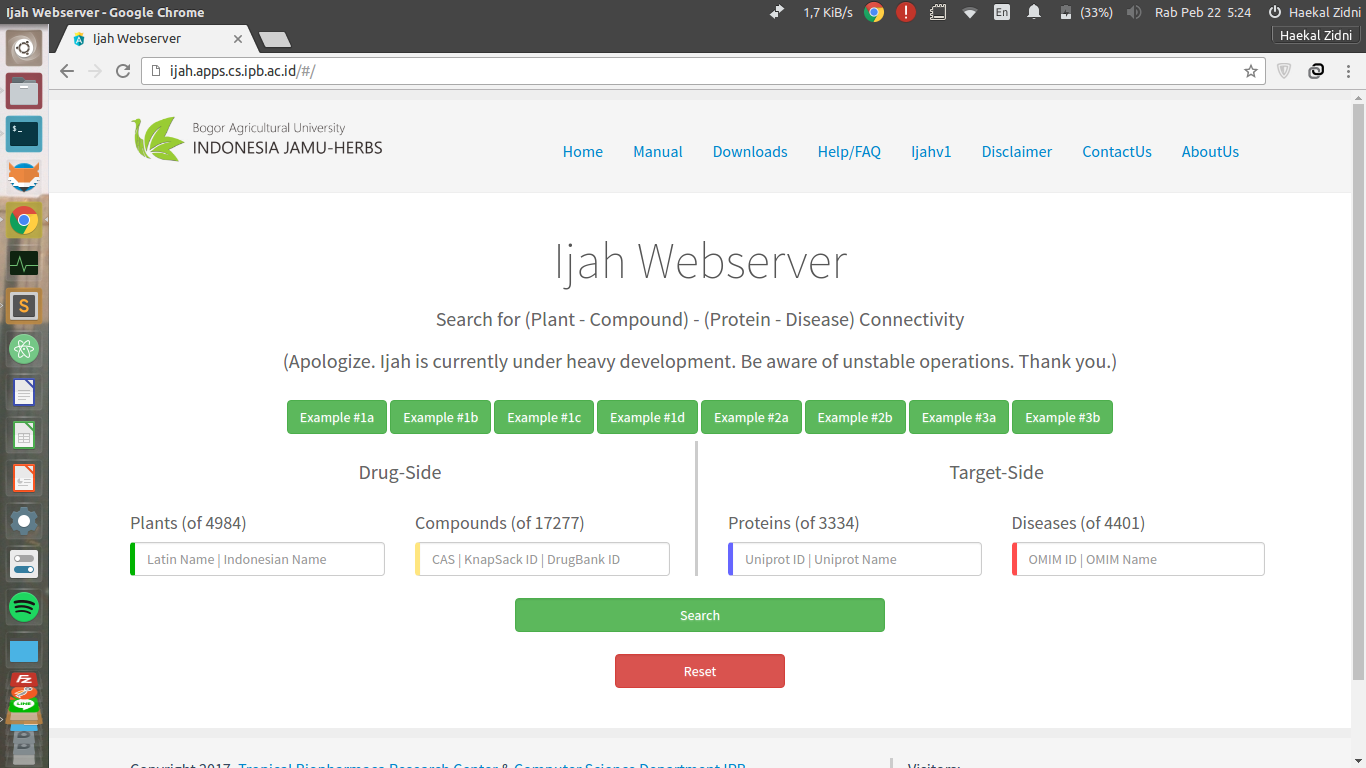
\includegraphics[scale=0.3]{ijah_startpage.png}
	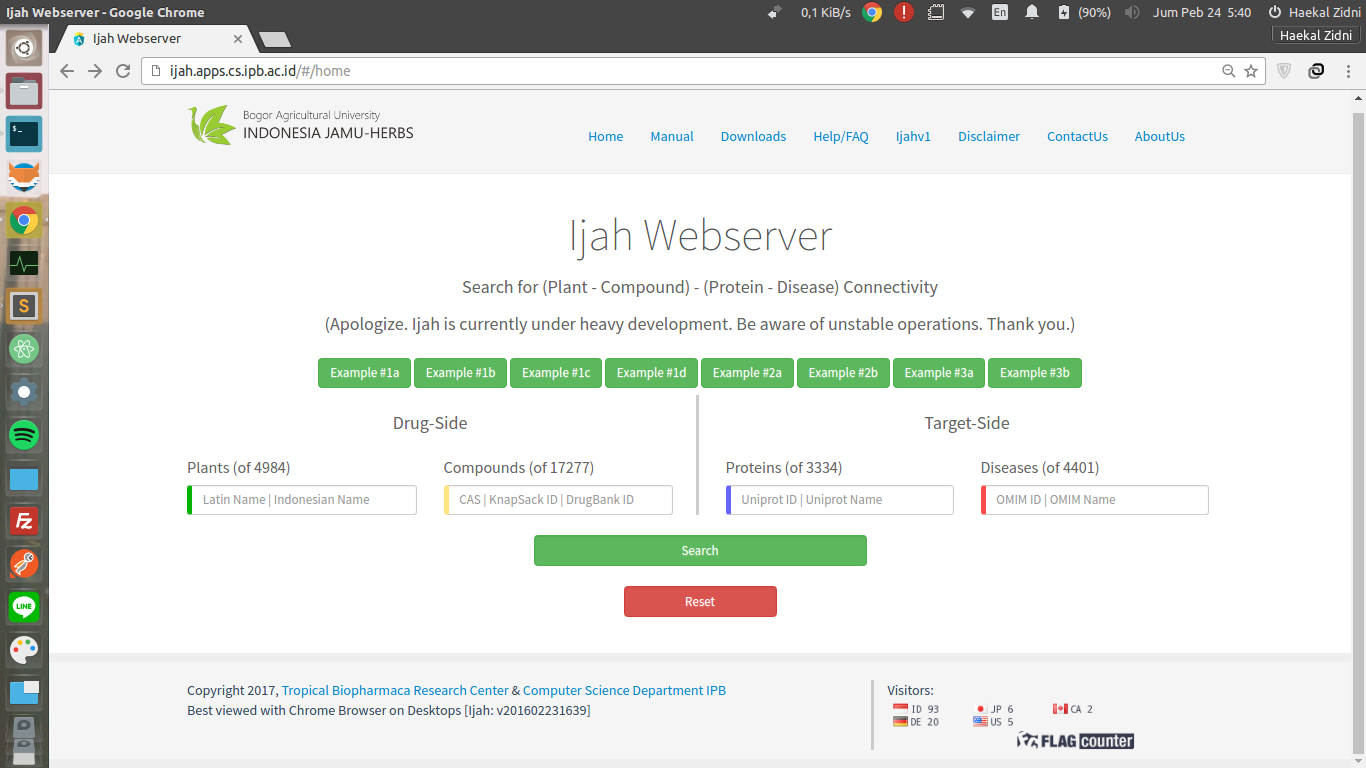
\includegraphics[scale=0.3]{ijah_full.png}
	\caption{Halaman utama Ijah Webserver}
	\label{fig:ijah_full}
\end{figure}

Pada bagian atas kanan halaman Ijah Webserver terdapat deretan menu. Deretan menu ini bisa diklik, dimana isi dan fungsi dari menu ini akan dijelaskan pada Bab \nameref{Menu}

\begin{figure}[!h]
	\centering
	
\includegraphics[scale=0.3]{ijah_menu_top.png}
	\caption{Deretan Menu pada Ijah Webserver}
	\label{fig:ijah_menu_top}
\end{figure}

Sedangkan pada bagian bawah Ijah Webserver terdapat Footer yang berisi \emph{version} Ijah Webserver yang berjalan dan \emph{Visitor Counter} yang berisi jumlah kunjungan Ijah Webserver berdasarkan negara pengunjung.

\begin{figure}[!h]
	\centering
	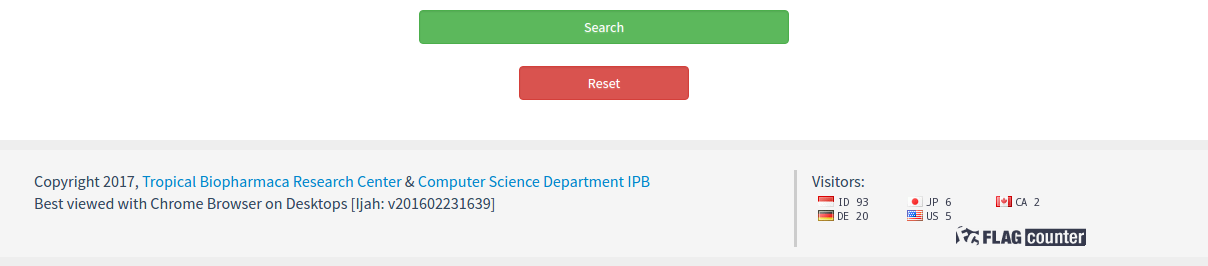
\includegraphics[scale=0.3]{ijah_footer.png}
	\caption{Posisi \emph{Visitor Counter} pada Ijah Webserver}
	\label{fig:ijah_footer}
\end{figure}

Pada nomor versi Ijah Webserver, 8 digit pertama merupakan format tahun-bulan-tanggal dan 4 digit terakhir merupakan jam dan menit. Sebagai contoh di Ijah Webserver v201702231639 berarti versi ini di-\emph{deploy} pada tanggal 23 Februari 2017 pukul 16:39.



Jika koneksi internet kurang memadai saat mengakses Ijah Webserver, kadang akan muncul kondisi sebagai berikut:

\begin{figure}[!h]
	\centering
	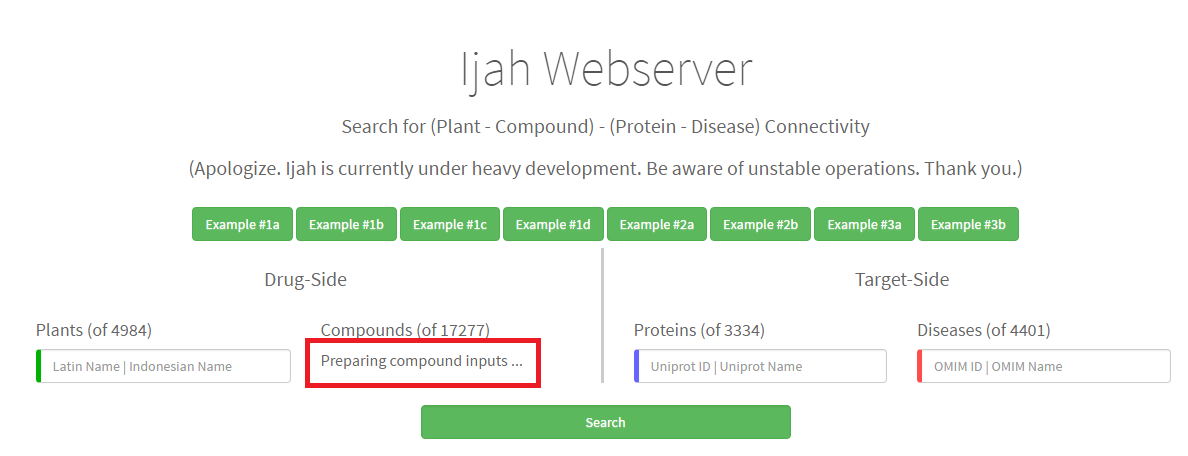
\includegraphics[scale=0.4]{ijah_prepare_output.png}
	\caption{Pesan yang muncul saat persiapan output belum selesai}
	\label{fig:ijah_prepare_output}
\end{figure}

Saat koneksi internet kurang memadai, ada kemungkinan muncul pesan ``Preparing compound inputs...'' artinya daftar input terkait sedang dimuat. Pada beberapa kondisi (misal internet kurang stabil) memang membutuhkan sedikit waktu untuk menyiapkan semua input.


